\hypertarget{_pixel_8hpp}{
\section{Pixel.hpp File Reference}
\label{_pixel_8hpp}\index{Pixel.hpp(145)@{Pixel.hpp(145)}}
}


\subsection{Detailed Description}
Declaration of the custom type Pixel. 



Definition in file \hyperlink{_pixel_8hpp-source}{Pixel.hpp}.

{\tt \#include $<$utility$>$}\par


Include dependency graph for Pixel.hpp:\nopagebreak
\begin{figure}[H]
\begin{center}
\leavevmode
\includegraphics[width=52pt]{_pixel_8hpp__incl}
\end{center}
\end{figure}


This graph shows which files directly or indirectly include this file:\nopagebreak
\begin{figure}[H]
\begin{center}
\leavevmode
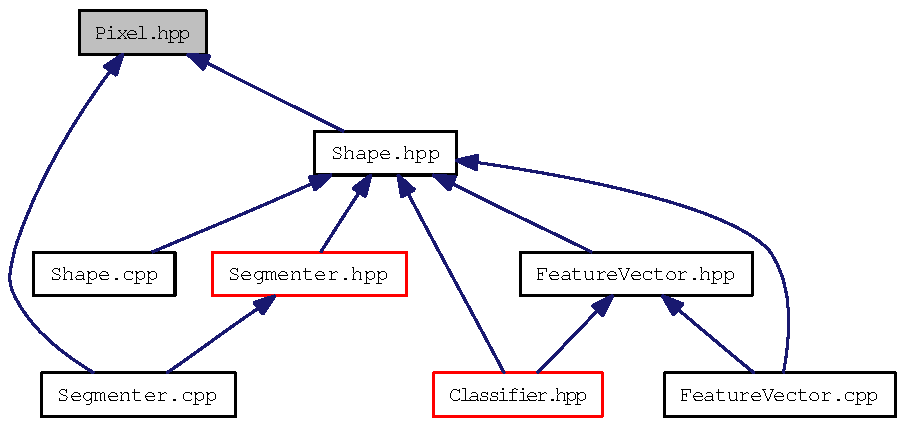
\includegraphics[width=234pt]{_pixel_8hpp__dep__incl}
\end{center}
\end{figure}
\subsection*{Typedefs}
\begin{CompactItemize}
\item 
typedef std::pair$<$ unsigned int, unsigned int $>$ \hyperlink{_pixel_8hpp_535e59456e3e633842529cfa8ea103c4}{Pixel}
\begin{CompactList}\small\item\em Information about an image pixel. \item\end{CompactList}\end{CompactItemize}


\subsection{Typedef Documentation}
\hypertarget{_pixel_8hpp_535e59456e3e633842529cfa8ea103c4}{
\index{Pixel.hpp@{Pixel.hpp}!Pixel@{Pixel}}
\index{Pixel@{Pixel}!Pixel.hpp@{Pixel.hpp}}
\subsubsection[Pixel]{\setlength{\rightskip}{0pt plus 5cm}{\bf Pixel}}}
\label{_pixel_8hpp_535e59456e3e633842529cfa8ea103c4}


Information about an image pixel. 

This pair keeps the coordinates of a pixel within a press clip. The first member representes the x coordinate (the row) and the second member representes the y coordinate (the column)

\begin{Desc}
\item[Author:]Eliezer Talón (\href{mailto:elitalon@gmail.com}{\tt elitalon@gmail.com}) \end{Desc}
\begin{Desc}
\item[Date:]2008-10-13 \end{Desc}


Definition at line 23 of file Pixel.hpp.